\documentclass[a4paper]{article}

%% Language and font encodings
\usepackage[english]{babel}
\usepackage[utf8x]{inputenc}
\usepackage[T1]{fontenc}
\usepackage{listings}

%% Sets page size and margins
\usepackage[a4paper,top=3cm,bottom=2cm,left=3cm,right=3cm,marginparwidth=1.75cm]{geometry}

%% Useful packages
\usepackage{amsmath}
\usepackage[colorinlistoftodos]{todonotes}
\usepackage[colorlinks=true, allcolors=blue]{hyperref}
\usepackage{listings}
\usepackage{url}
\usepackage{graphicx}
\graphicspath{ {./images/} }
% \DeclareGraphicsExtensions{.pdf,.jpg,.png}

%% defined colors
\definecolor{Blue}{rgb}{0,0,0.5}
\definecolor{Green}{rgb}{0,0.75,0.0}
\definecolor{LightGray}{rgb}{0.6,0.6,0.6}
\definecolor{DarkGray}{rgb}{0.3,0.3,0.3}

% \newcommand*\lstinputpath[1]{\lstset{inputpath=#1}}
% \lstinputpath{code/}

\lstset{language=R,
   basicstyle=\ttfamily\small,
   breaklines=true,
   keywordstyle=\bfseries\color{Blue},
   commentstyle=\itshape\color{LightGray},
   stringstyle=\color{Green},
   numbers=left,
   numberstyle=\tiny\color{DarkGray},
   stepnumber=1,
   numbersep=10pt,
   backgroundcolor=\color{white},
   tabsize=2,
   showspaces=false,
   showstringspaces=false,
   captionpos=b,
%    inputpath={code/},
   frame=tb
}

\lstset{language=Python,
   basicstyle=\ttfamily\small,
   breaklines=true,
   keywordstyle=\bfseries\color{Blue},
   commentstyle=\itshape\color{LightGray},
   stringstyle=\color{Green},
   numbers=left,
   numberstyle=\tiny\color{DarkGray},
   stepnumber=1,
   numbersep=10pt,
   backgroundcolor=\color{white},
   tabsize=2,
   showspaces=false,
   showstringspaces=false,
   captionpos=b,
%    inputpath={code/},
   frame=tb
}

\lstset{language=Matlab,
   basicstyle=\ttfamily\small,
   breaklines=true,
   keywordstyle=\bfseries\color{Blue},
   commentstyle=\itshape\color{LightGray},
   stringstyle=\color{Green},
   numbers=left,
   numberstyle=\tiny\color{DarkGray},
   stepnumber=1,
   numbersep=10pt,
   backgroundcolor=\color{white},
   tabsize=2,
   showspaces=false,
   showstringspaces=false,
   captionpos=b,
%    inputpath={code/},
   frame=tb
}

\title{Assignment 3: Missing Data Tutorial}
\author{
Low, Daniel Mark (S3120155) \\
Petre, Bogdan (S3480941) \\
Xu, Teng Andrea (S3548120) \\ 
 \\ \textbf{Group} 7}
\date{\today}


\begin{document}
\maketitle

%\todo{Group is combined with author which is somewhat clumsy. }
%\todo{Let me know what you think.}
%\todo{Daniel: I think it is fine.}

\section*{Introduction and Motivation}
Missing data is everywhere. You are likely to find it in any dataset you want to analyze. Why is missing data a problem? One of the main issues is obtaining biased results from statistical tests such as correlation. For instance, perhaps two variables would not correlate as much if the missing data was available. 
This is a tutorial covering the basic and more advanced methods for dealing with missing data. We provide all code in a jupyter notebook available at this link: 

\url{https://github.com/bogdanp05/IDS_Assignment2}

\par\noindent First, we will explain the different types of missingness you might encounter with examples of each. Then, we will provide basic methods for handling missing data, including discarding data and single value imputation with implementations in Python. Finally, we will review more advanced methods, such as multiple value imputation with implementations in R so we can end by comparing both languages in handling missing data.
These methods are dealing with a problem, which is that somehow data was lost or never obtained. Therefore, the first rule of dealing with missing data is to avoid missing data in the first place. Extra care should be taken during data collection to avoid missingness as much as possible.

\section{Relevant bibliography}
1. Gelman and Hill (2007) \cite{Gelmann}.
Comment: We used Chapter 25 of this book which covers most of what we included in our tutorial.

\par\noindent 2. Azur et al. (2011) \cite{MICE}. 
Comment: This paper reviews the theory behind Multiple Imputation.

\par\noindent 3. Therese D. Pigott (2001) \cite{AReviewofMethods}.
Comment: Deepening the differences between Multiple Imputation and Single Imputation.

\par\noindent 4. Marina Soley-Bori (2013) \cite{Dealingwith}.
Comment: Chapter 4 of the paper explains the most used techniques in order to deal with missing data.

\section{Types of missing data}
\par\noindent There are four main types of missing data that occur in data sets \cite{Gelmann}.\\

\par\noindent \textbf{Missingness completely at random} is when there is the same chance of having missing values for all units. You would end up with the same statistical results with the true data as with this type of missing data. 
\par\noindent \textit{Example 1:} If there is a survey where the participants have to regularly submit some data, we could have missing values because sometimes people simply forget to submit.
\par\noindent \textit{Example 2:} We could have an old data set (like the Titanic data set) in which some of the values got damaged beyond recognition (e.g., ink wearing off).\\

\par\noindent \textbf{Missingness at random} is when the chance of a variable to be missing depends only on other, fully recorded variables.
\par\noindent \textit{Example:} In a survey where age and education are fully recorded, we could say that the \textit{income} variable is missing at random if the chance of missingness depends only on these other variables, which have no missing values.\\

\par\noindent \textbf{Missingness that depends on unobserved predictors} is when the chance of a recorded variable to have missing values depends on variables that are not recorded. This case is similar to the \textit{missingness at random} case, with the exception that the variables indicative of the variable of interest are not recorded.
\par\noindent \textit{Example:} Imagine a survey where a variable is represented by the answer to a complicated question. Non native speakers might have trouble understanding the question and may therefore not respond to it. If the country of origin is not recorded, then the missingness depends on unobserved predictors.\\

\par\noindent \textbf{Missingness that depends on the missing value itself} is when the chance of a variable to be missing depends on the value of that variable.
\par\noindent \textit{Example 1:} A classic example is that people with higher incomes tend to not state their income.
\par\noindent \textit{Example 2:} A more recent example of this phenomena was during the US presidential election of 2016, when, during the polls before the election, a lot of Donald Trump supporters declined to answer out of social embarrassment.\\

\par\noindent \textit{Question:} Which of these types of missing data is the most desirable?
\par\noindent \textit{Answer: } The ideal case is that of Missingness Completely at Random (the types of missing data are actually ordered from best to worst case scenario) because the variable has the same probability to be missing for all the records variables. A good way to deal with it would be to simply remove the rows entirely, since this will not bias the results, which would lead to what is called Complete-Case Analysis. However, in most cases it is impossible to prove the complete random nature of a missing variable. What data scientists try to do instead is to create a model for this variable and to include as many observed predictors as possible (e.g., create a model for income that takes into account age, gender, education, region).

\section {Visualizing your (missing) data}

For this tutorial, we will use the Titanic dataset, a widely used dataset in Data Science. It has information on 1300 passengers of the Titanic, including their names, age, if they survived, where they were heading, and other relevant information. We will use Pandas, which is a Python library for easily manipulating dataframes. We will also use matplotlib, which is for plotting visualizations.
The first step is to import the libraries and the Titanic dataset. Then we are going to print the first 20 rows using the DataFrame.head(n) method. Pandas prints the last columns below.

\begin{figure}[ht!]
\centering
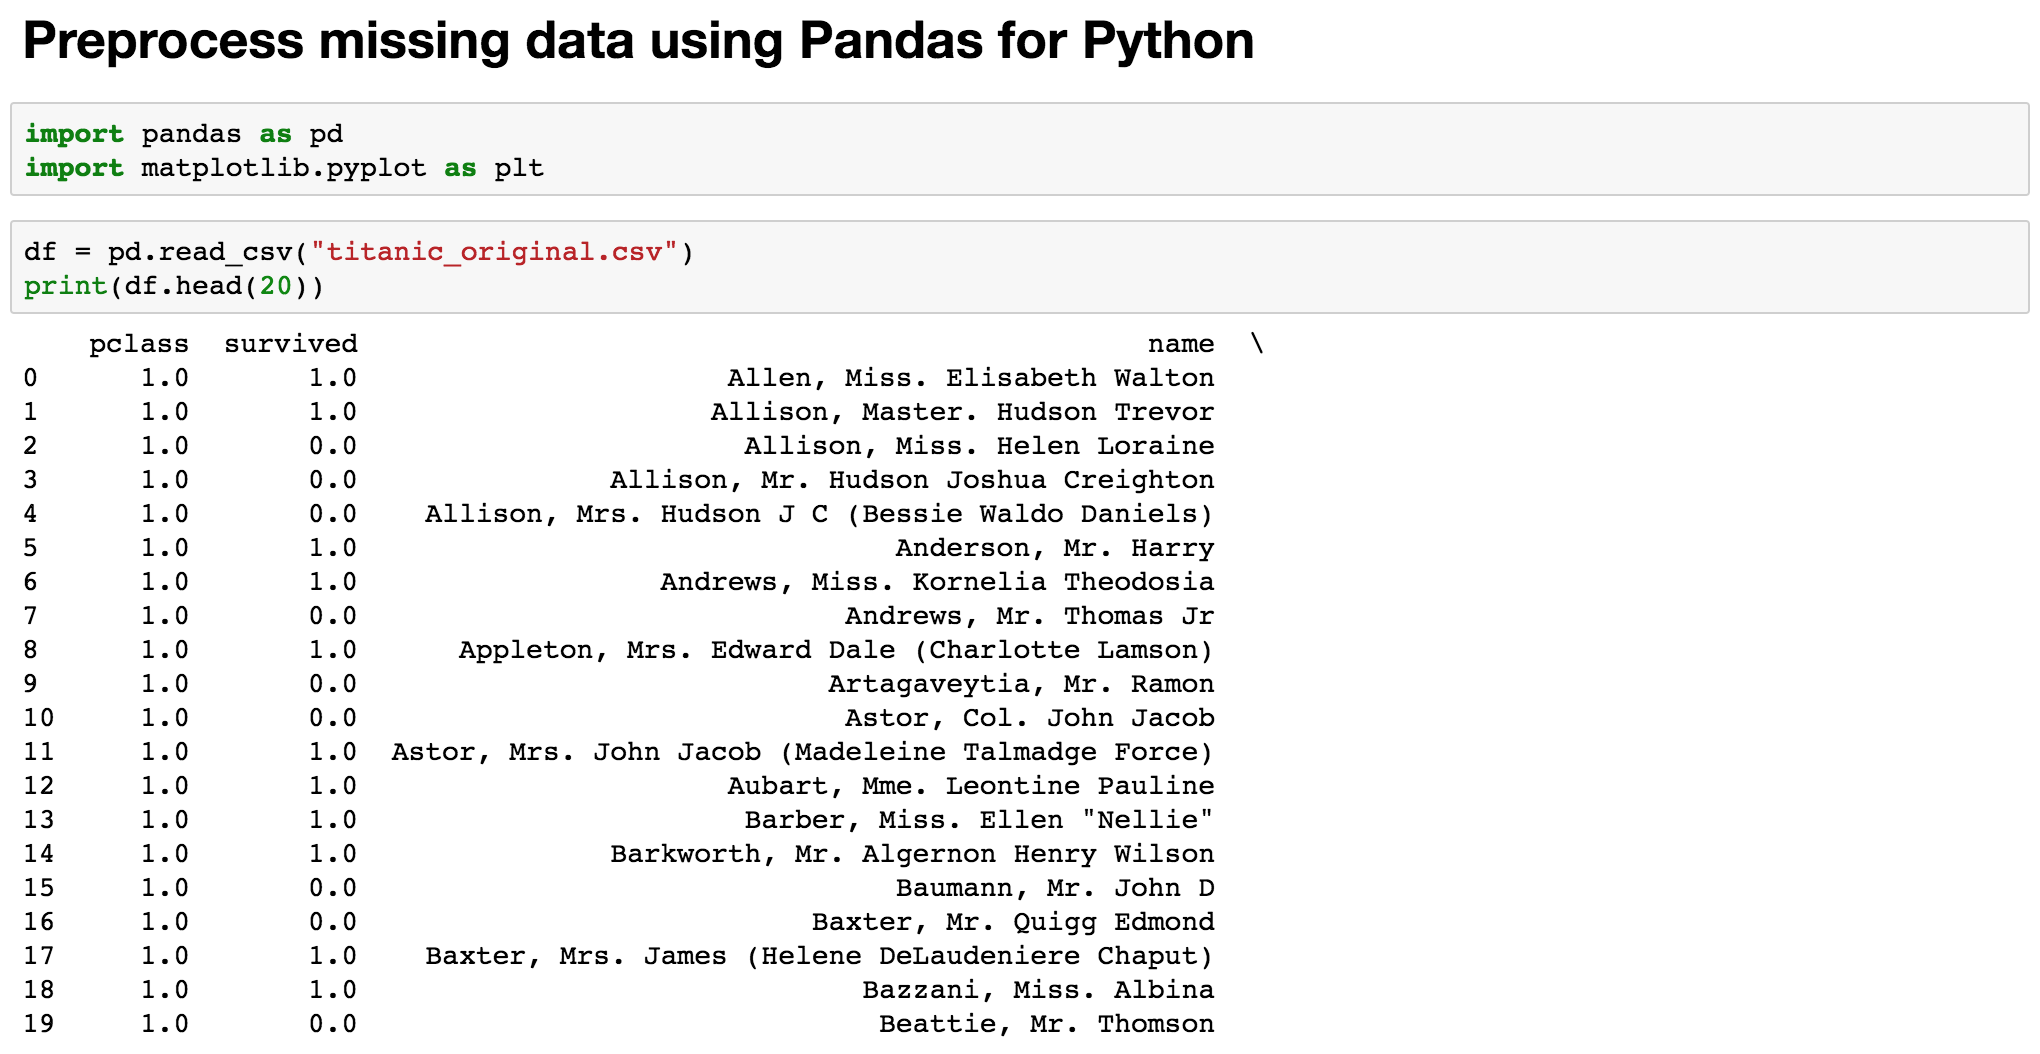
\includegraphics[width=0.9\textwidth]{images/python1.png}
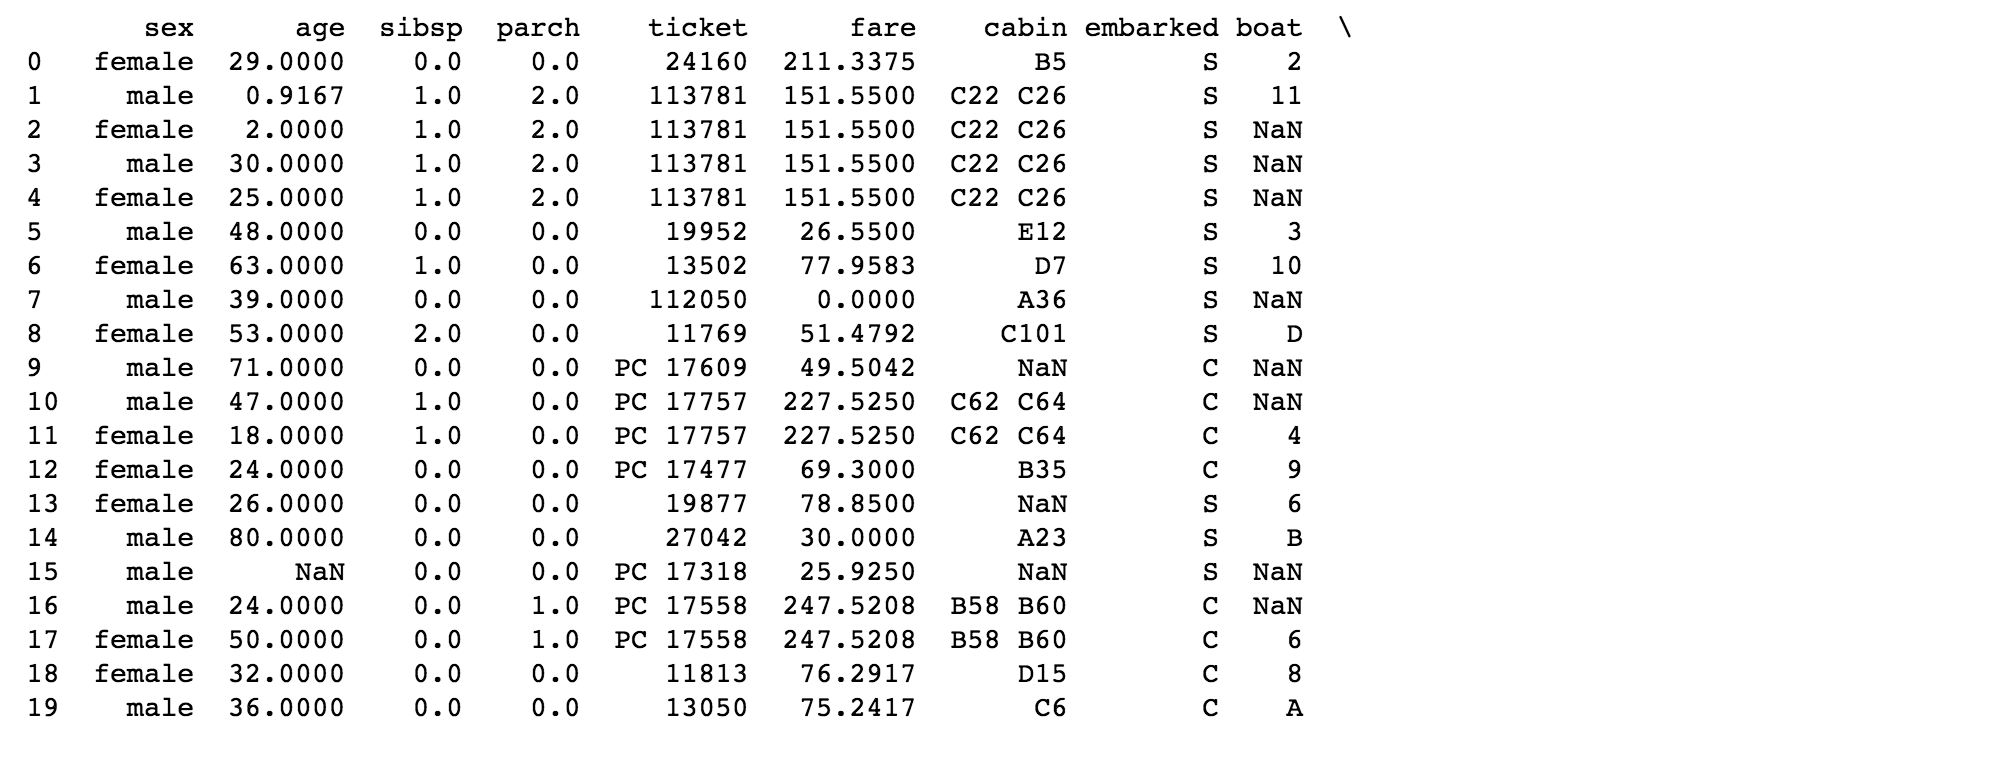
\includegraphics[width=0.9\textwidth]{images/python1b.png}
\caption{Importing the libraries and the Titanic dataset}
\end{figure}

\pagebreak\par\noindent Then we use a Python dictionary to make a bar plot. As we can see, variable Age has over 200 missing data. 

\begin{figure}[ht]
\centering
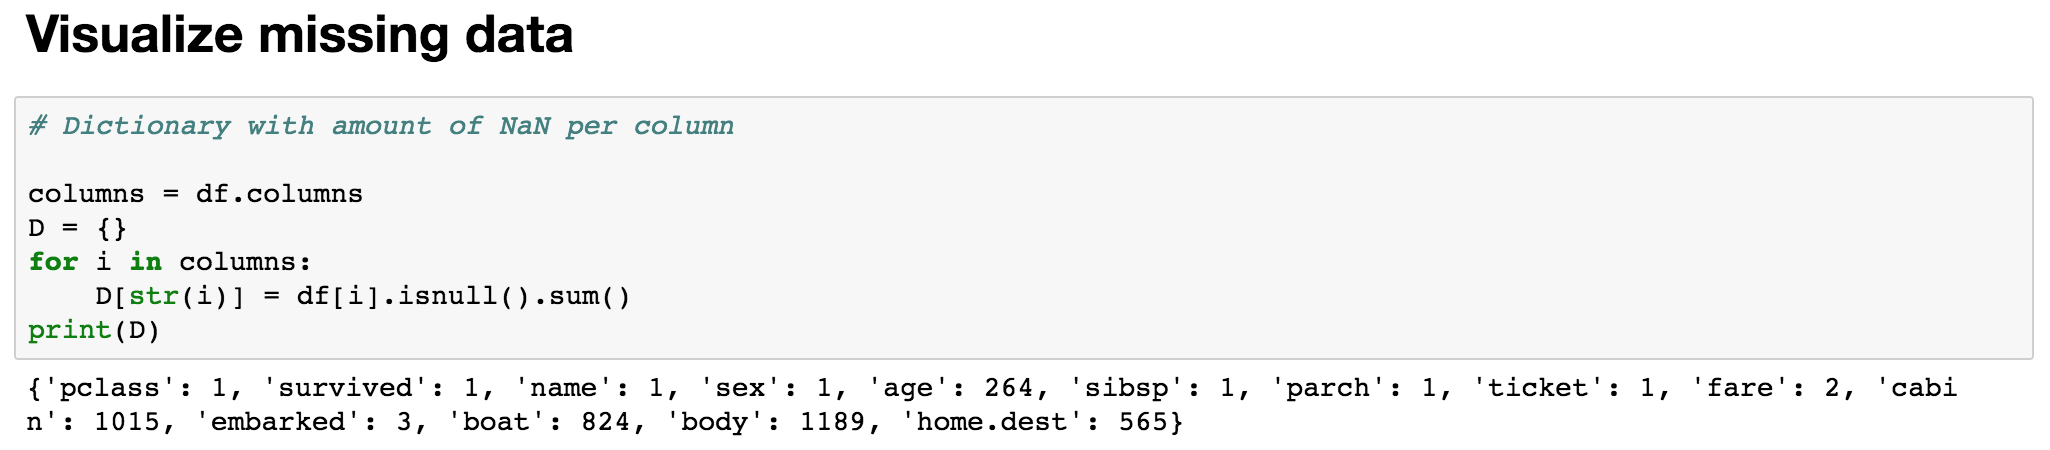
\includegraphics[width=\textwidth]{images/python2.png}
\caption{Python dictionary}
\end{figure}

\begin{figure}[ht]
\centering
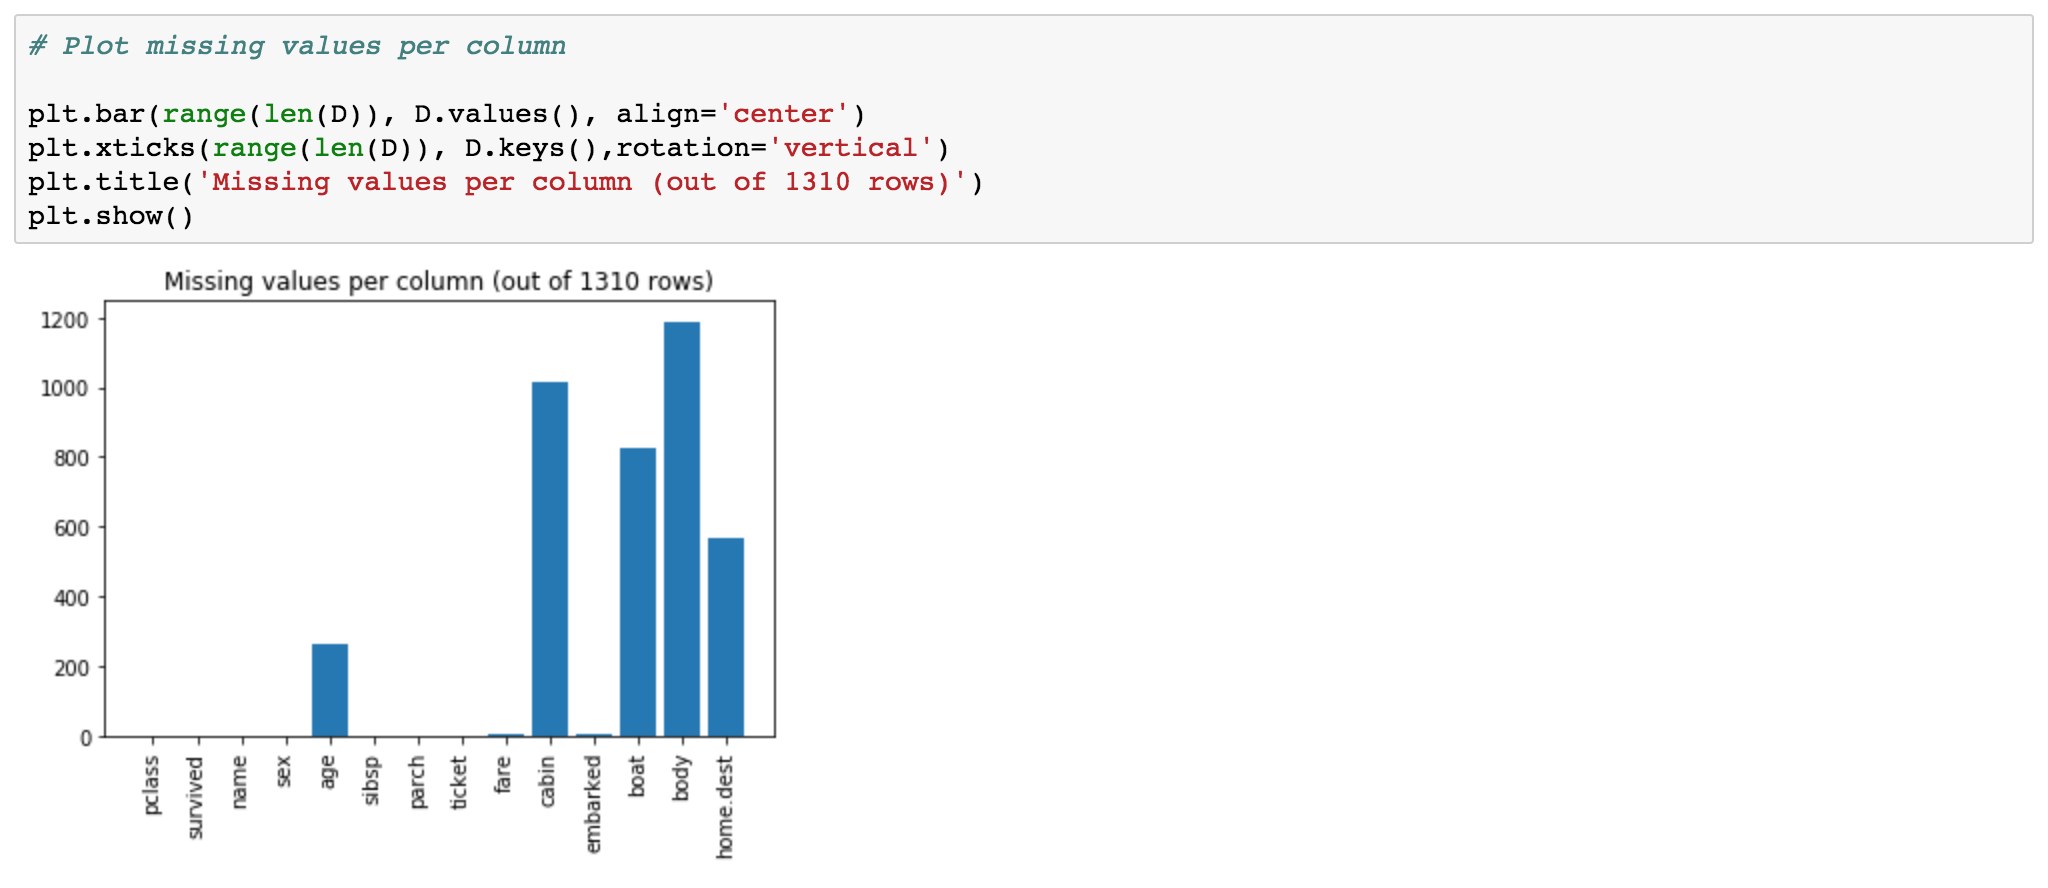
\includegraphics[width=\textwidth]{images/python3.png}
\caption{Bar plot of missing data per variable}
\end{figure}

\pagebreak\par\noindent Now we can start looking at possible solutions.

\section{Discarding missing data}

One solution is to discard every row where there is at least one missing value. This is the complete-case analysis mentioned before. 

\begin{figure}[htbp]
\centering
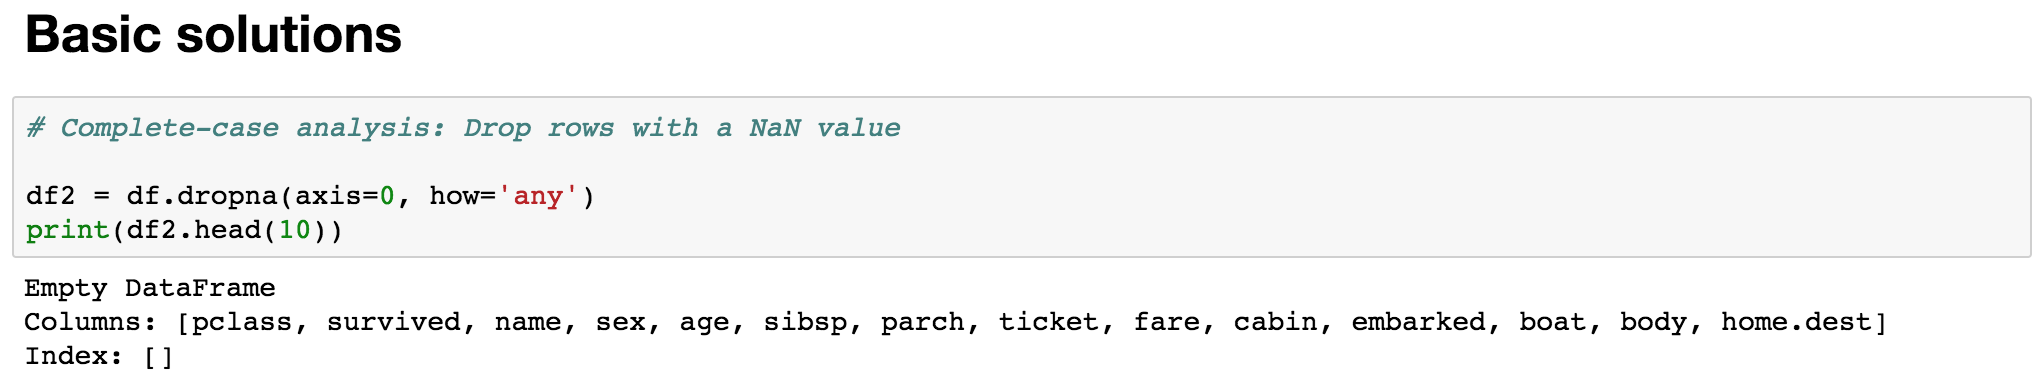
\includegraphics[width = \textwidth]{images/python4a.png}
\caption{Complete-case analysis: discard rows with missing data}
\end{figure}

\par\noindent The result is an empty dataframe! All rows in this dataset have at least one missing value in a given variable. 

\par\noindent \textit{Question: } When can I use complete-case analysis work?
\par\noindent \textit{Answer: }When the records with missing values do not differ dramatically from the ones with recorded values and when the number of rows to be dropped is relatively small (e.g., ~5\%).

\section*{Single value imputation}

Another solution is to perform an imputation or fill-in a missing value with another value. Which value should be used? The mean of the variable is commonly used. Row 15 was NaN before and now it is filled. 

\begin{figure}[htbp]
\centering
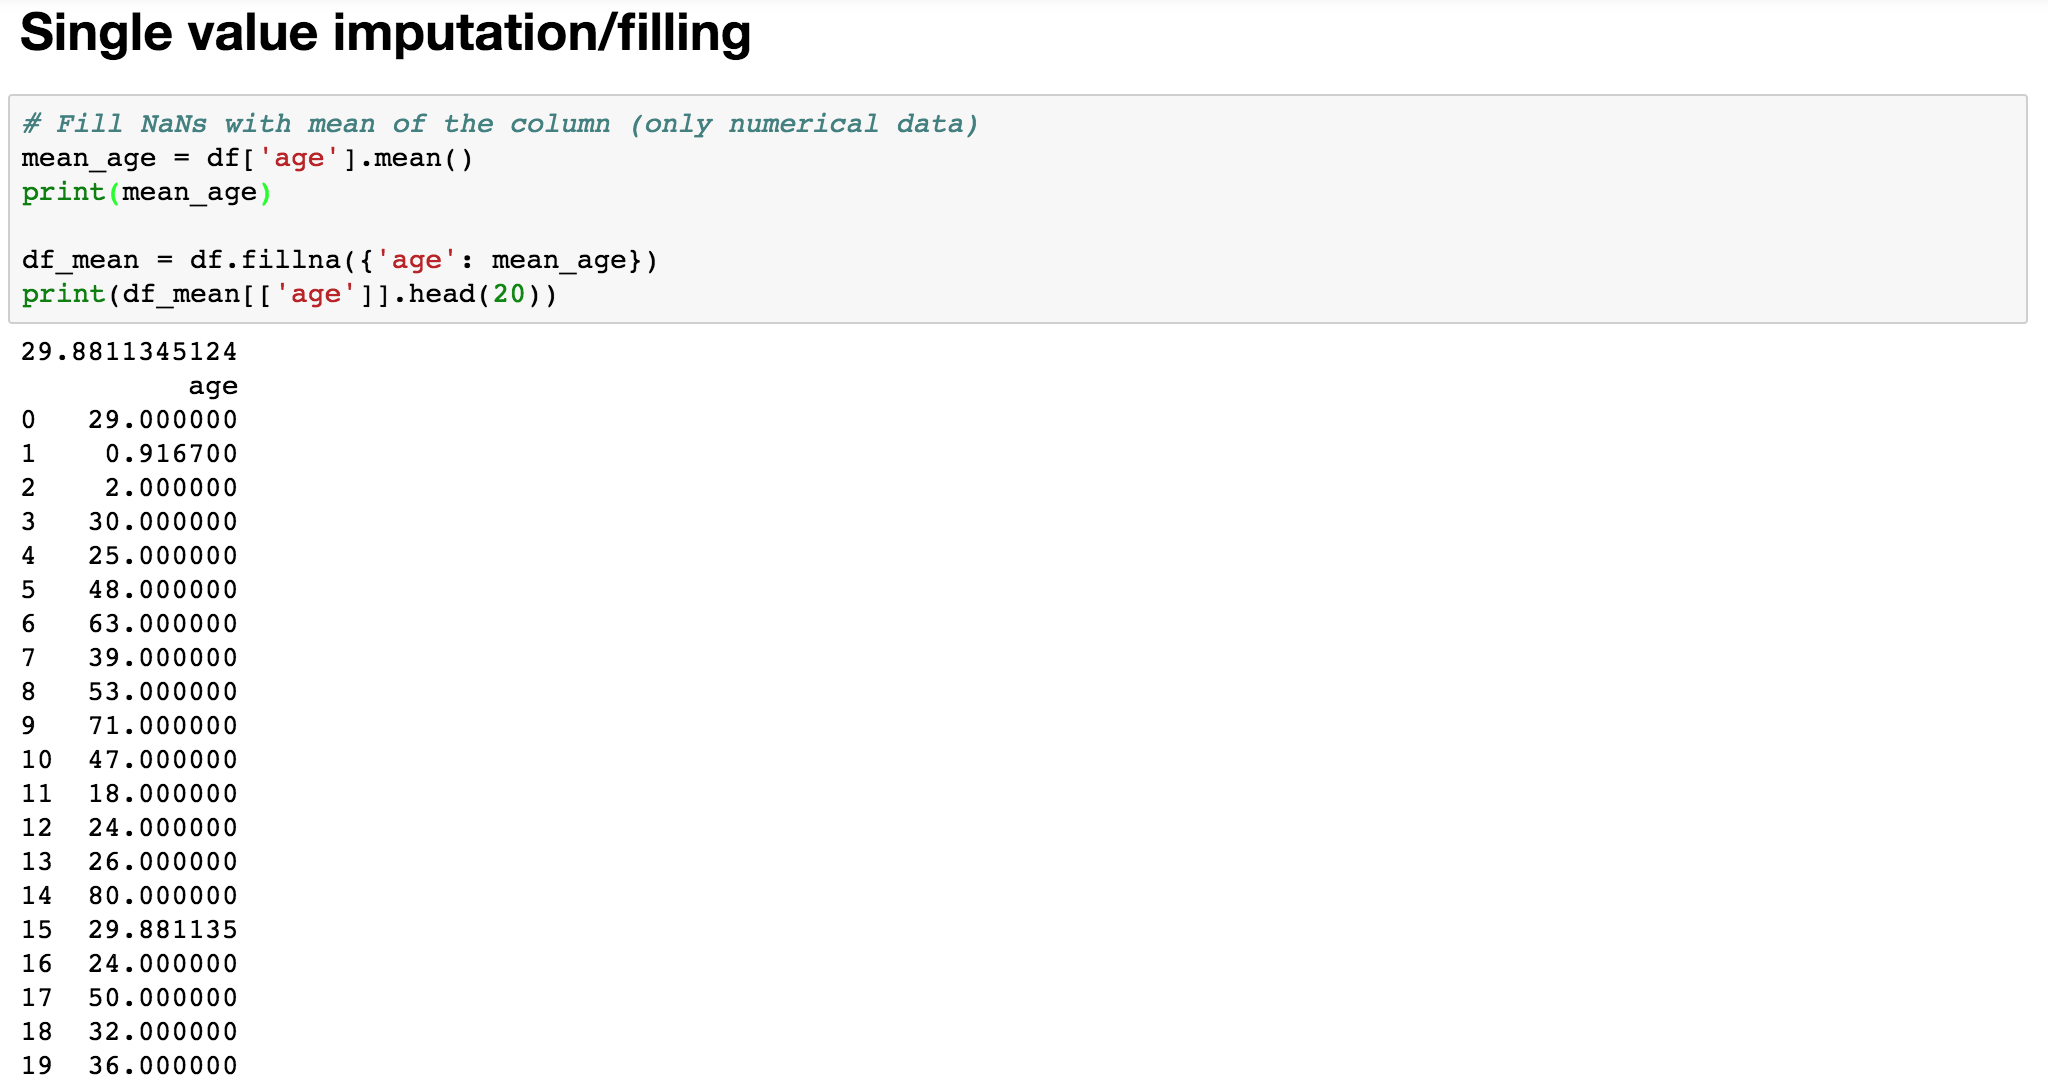
\includegraphics[width = \textwidth]{images/python4.png}
\caption{Replacing missing data with the mean}
\end{figure}

\par\noindent Just to show that it worked, we can plot the amount of missing data per variable again and see that Age dropped to zero missing values. 

\begin{figure}[htbp]
\centering
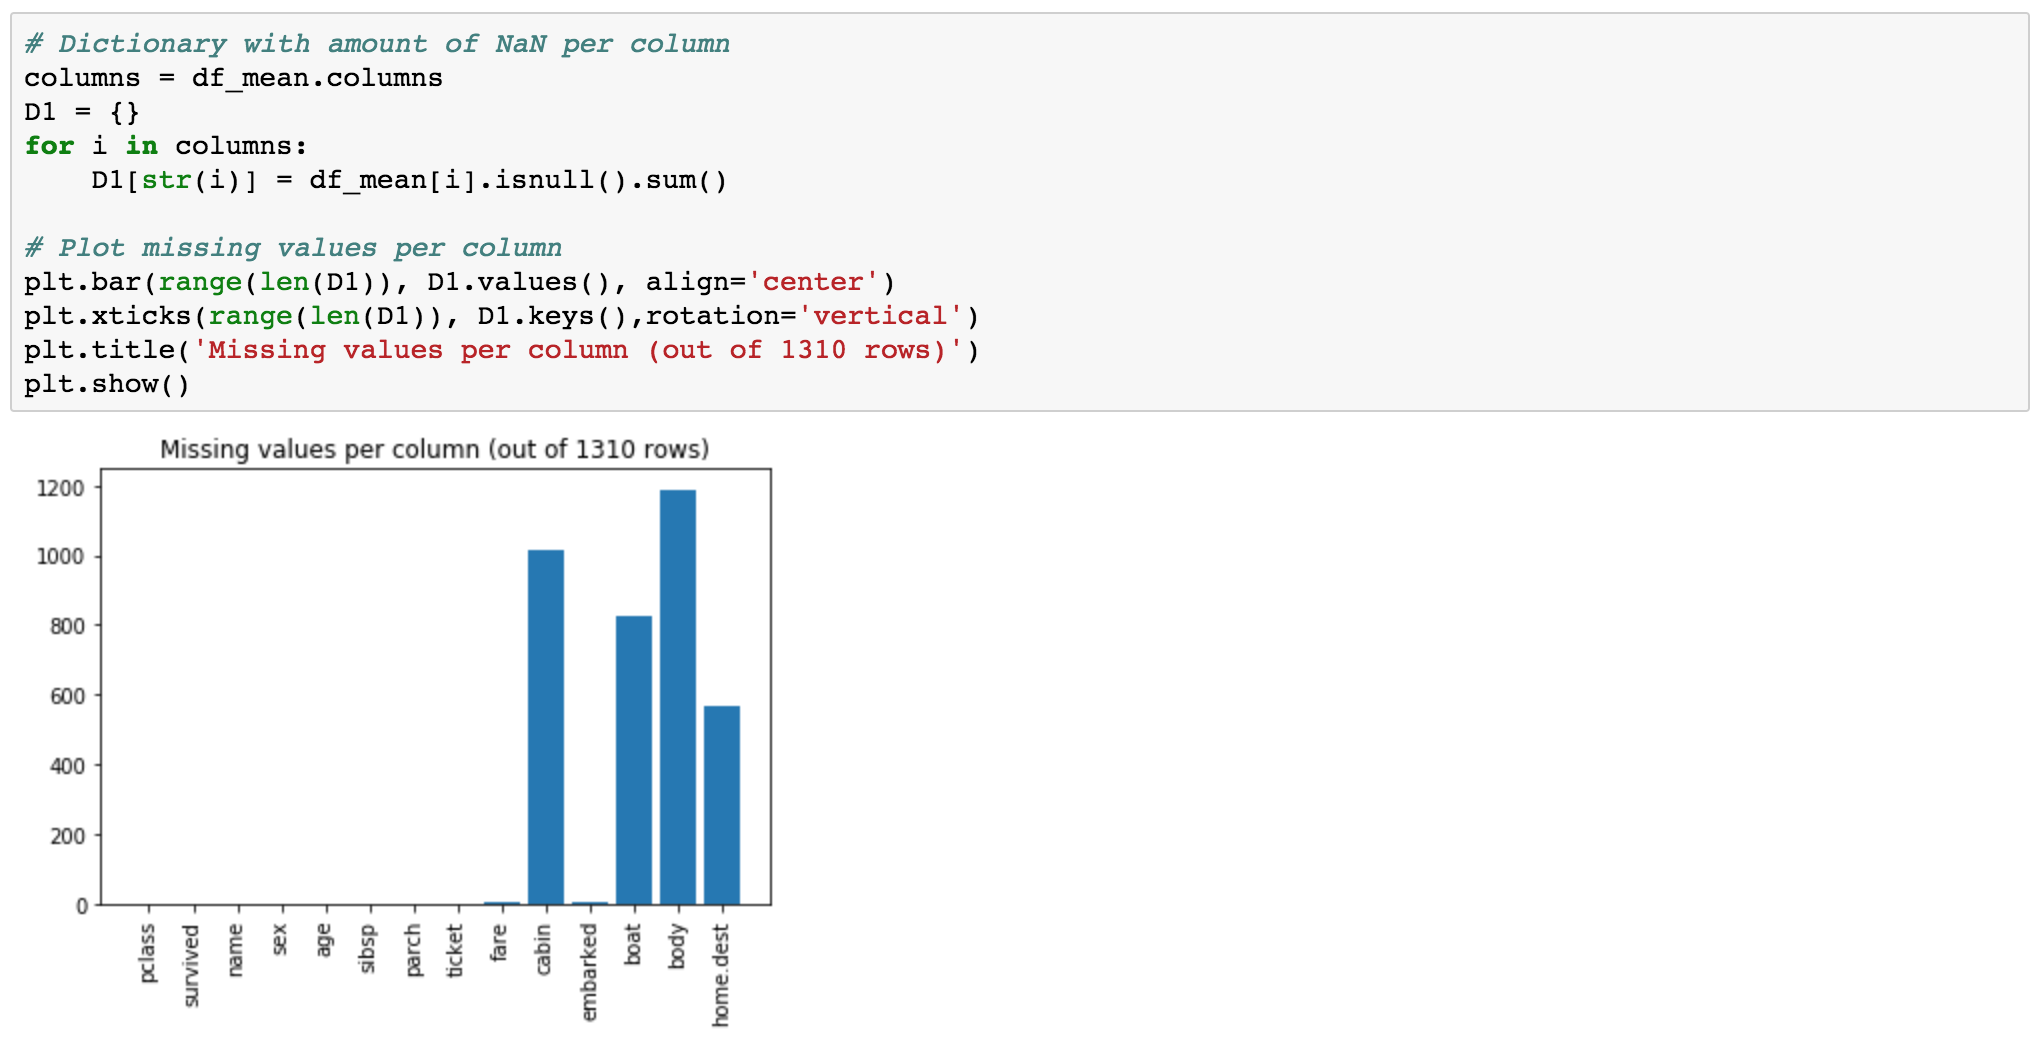
\includegraphics[width = \textwidth]{images/python5.png}
\caption{Bar plot of missing data per variable}
\end{figure}

\par\noindent The problem with imputing the mean is that the mean is not always a good approximation. It does not really make sense to replace the age of a passenger with ~29.8. It also has the drawback of reducing the correlations between variables. Furthermore, it underestimates the true variance, which is used to compute statistical tests. This will result in biased data. We can compute the standard deviation to demonstrate this.\\

\begin{figure}[htbp]
\centering
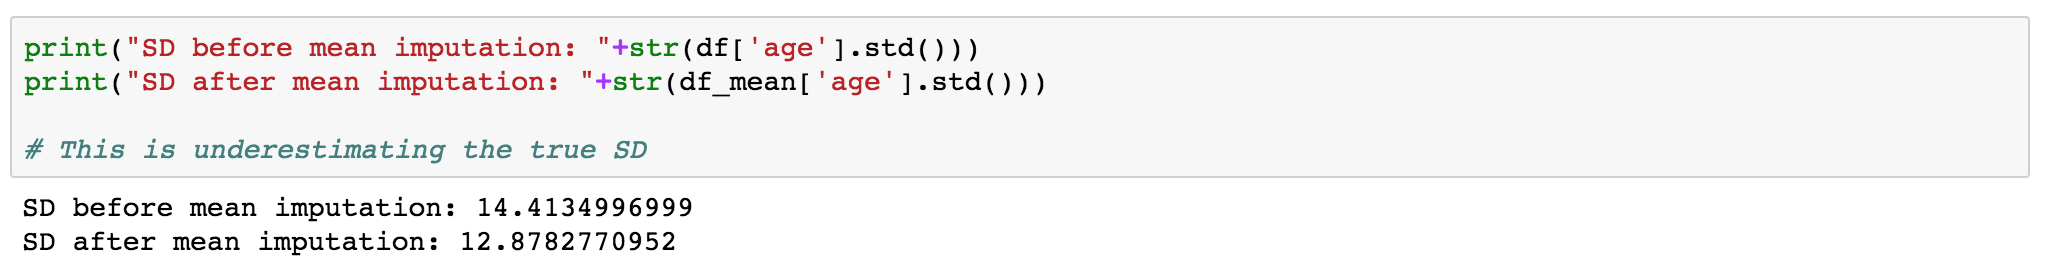
\includegraphics[width = \textwidth]{images/python6.png}
\caption{Standard deviation before and after imputing the mean}
\end{figure}

\par\noindent \textit{Question: } When can I use single imputation with the mean? 
\par\noindent \textit{Answer: } If there is a variable with low variance then the mean will be a good approximation. For example, if there is a reaction time experiment the require a button press, and some instances were not recorded and there is low variance, then the mean may be a good substitute.\\ 

\par\noindent Another type of single value imputation is filling in the value with the value after the missing value --backward filling-- or with the value before this missing value --forward filling--. We can see that row 15 is now filled-in.

\begin{figure}[htbp]
\centering
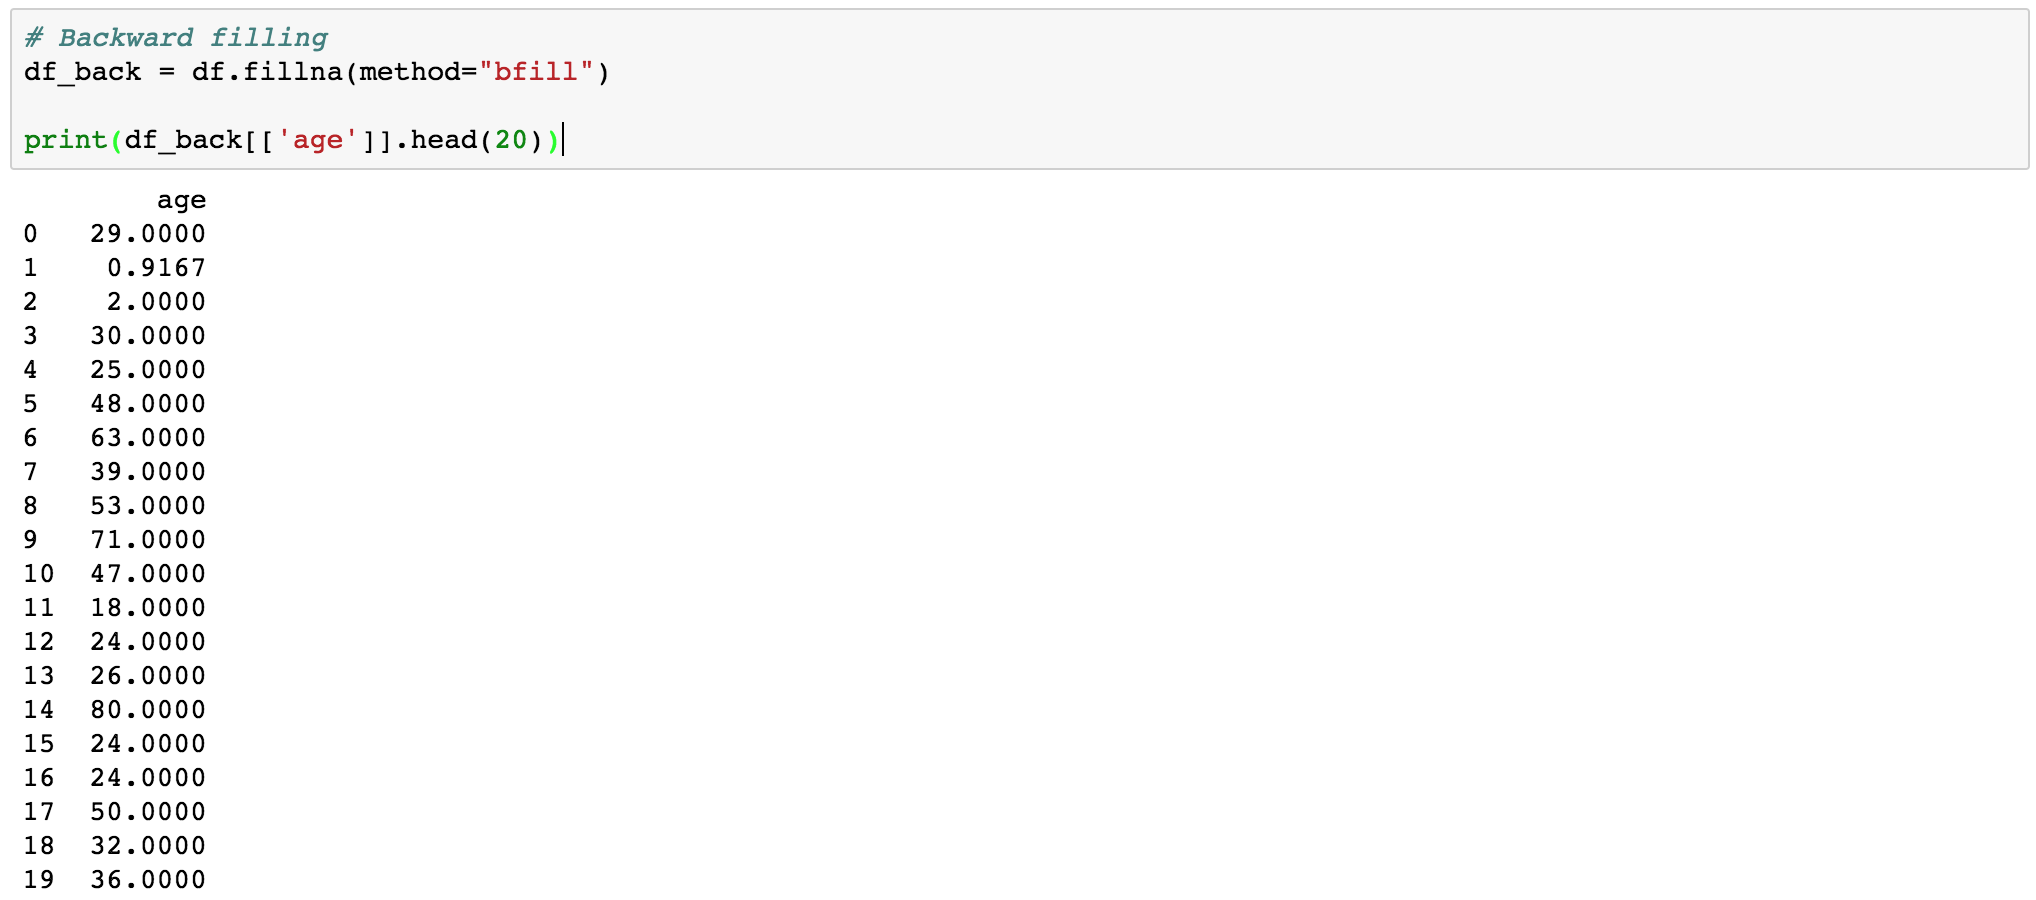
\includegraphics[width = \textwidth]{images/python7.png}
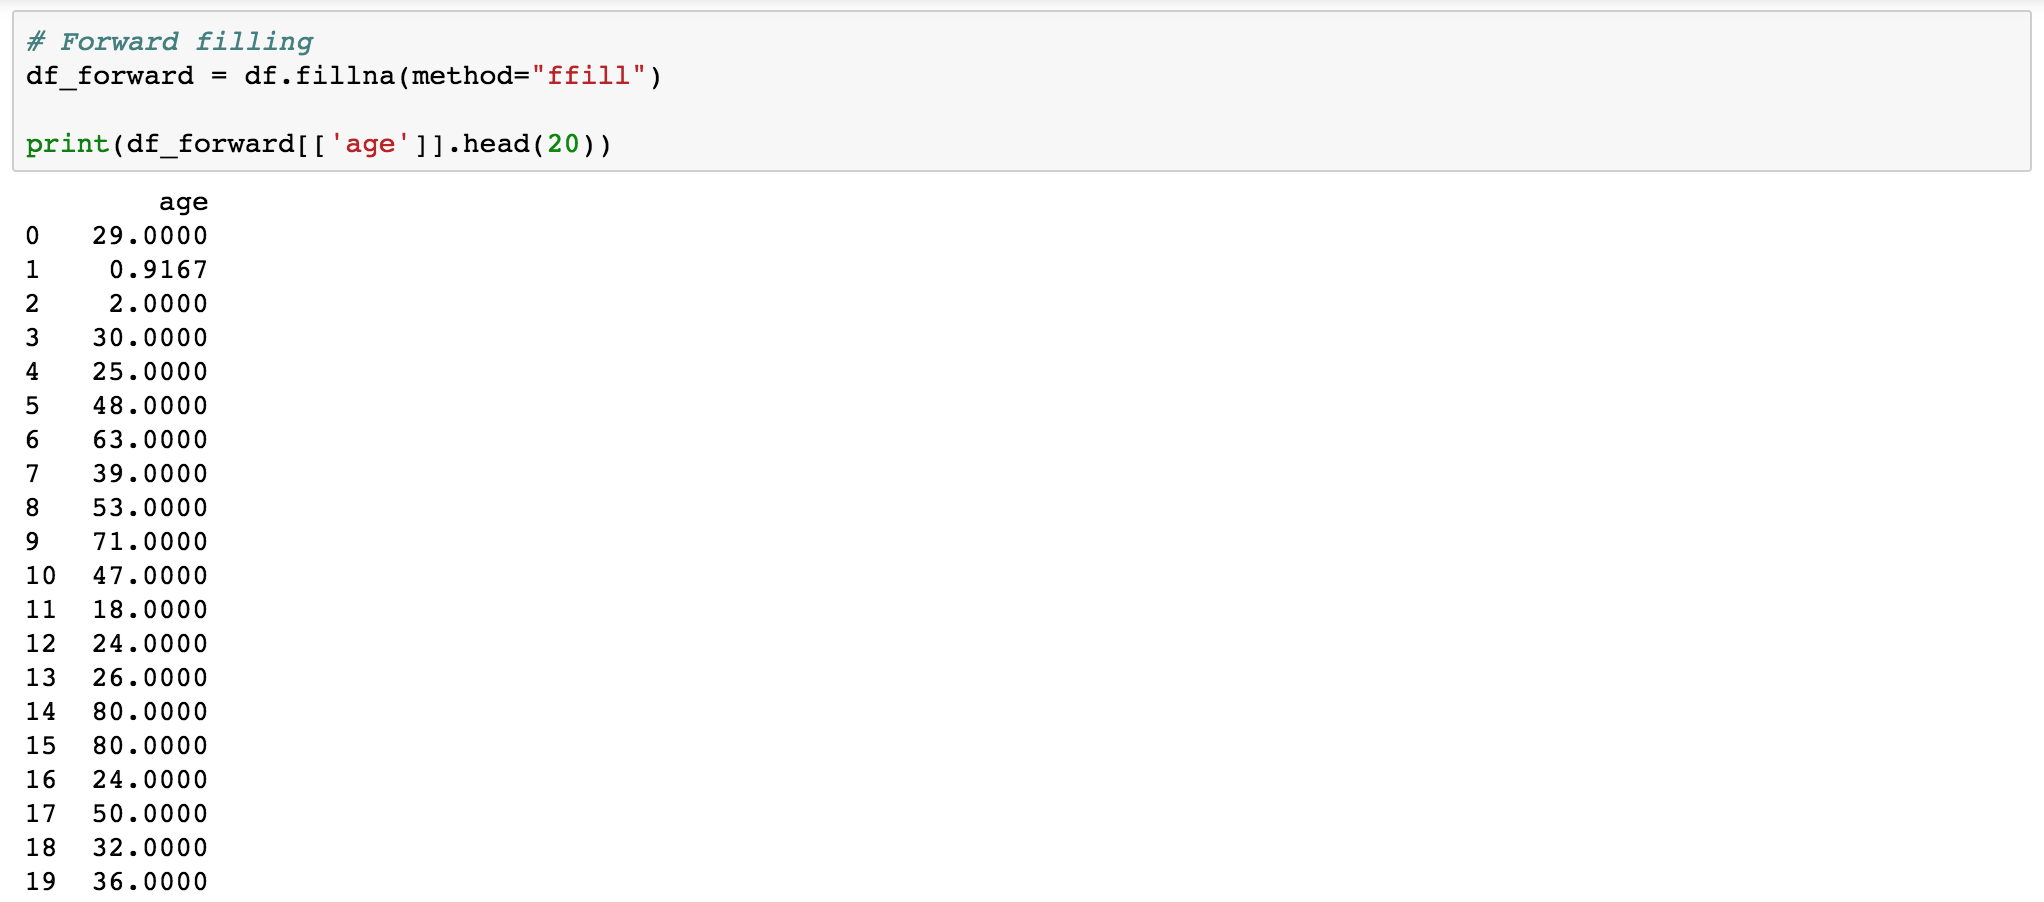
\includegraphics[width = \textwidth]{images/python8.png}
\caption{Backward and forward filling}
\end{figure}

\par\noindent The issue with forward and backward filling is that suppose that value around a NaN is an outlier (e.g., Age = 91). Then we would be duplicating the outlier, which could affect our ability to detect outliers and would also affect the mean. Perhaps this method might be useful if data is ordered along a certain variable, for instance, "Position in race". If one knows that subject in 4th place arrived almost at the same time as subjects in 3 or 5th place (which is common in short track competitions), then one could impute using this method. But be careful and analyze your specific case. 

\section{Multiple Value Imputation}

Another approach used in order to deal with missing data is the Multiple Imputation technique. This approach as opposed to single imputation, accounts for the statistical uncertainty in the imputations.\cite{MICE}\\
This is done by creating several imputed values --not just one-- for each missing value, each of which is predicted for a slightly different model and each of which also reflects sampling variability.\cite{Gelmann}\\
At the end of the process we will have multiple "complete" datasets in which we are able to calculate variance and infer which of the new data values is better suited to replace the missing value.\\
The goal of Multiple Imputation is not to re-create the individual missing values as close as possible to the true ones, but to handle missing data to achieve valid statistical inference.\cite{Dealingwith}\\
In the following example, we will show how multiple imputation works using R as a programming language with the well documented library MICE. The MICE library is a set of functions that deal with missing data and are able to deal with numerical values with different algorithms (e.g., "pmm"(predictive mean matching), "rd"(Random Forest), "norm" (Bayesian Linear Regression), among others).\\
Furthermore, categorical types of data can also be predicted using algorithms like "logreg"(Logistic Regression) or "polyreg" (Polytomous Logistic Regression).\\
N.B: In order to use these methods, the data has to be factorized in order to enable machine learning on each category.\\
 
 \subsection*{Demonstration}
 We worked with the Titanic dataset and we will fill in a specific type of entry that is currently missing, in this case, Age.
 
\begin{figure}[htbp]
\centering
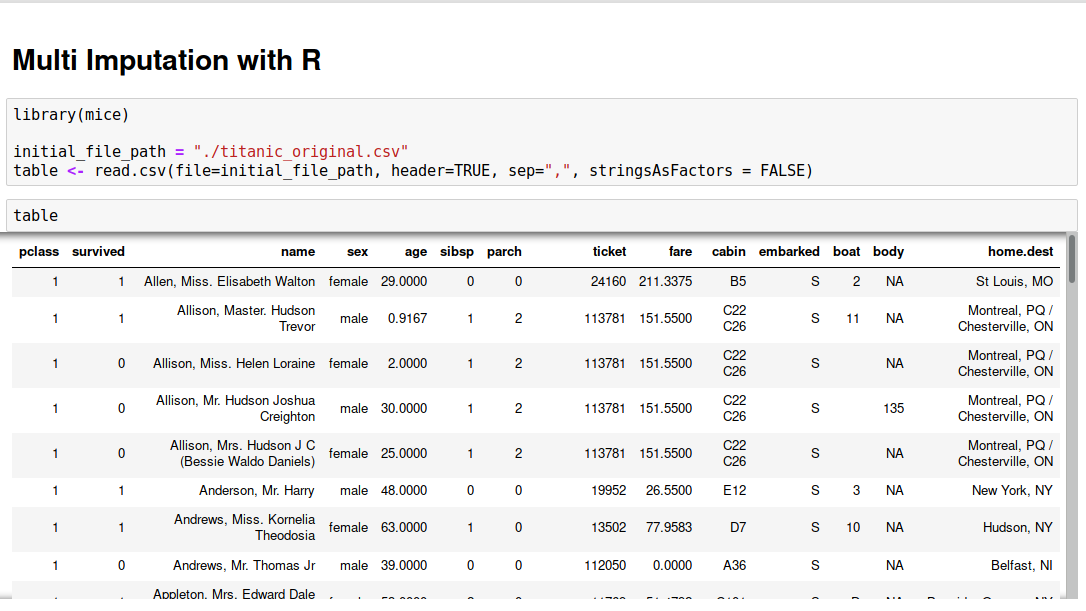
\includegraphics[width = \textwidth]{images/R1.png}
\caption{Importing the titanic dataset}
\end{figure}
\newpage
\par\noindent After we imported our table to work on, we can analyze it, as always, to see how many entries are missing for each column.
\begin{figure}[htbp]
\centering
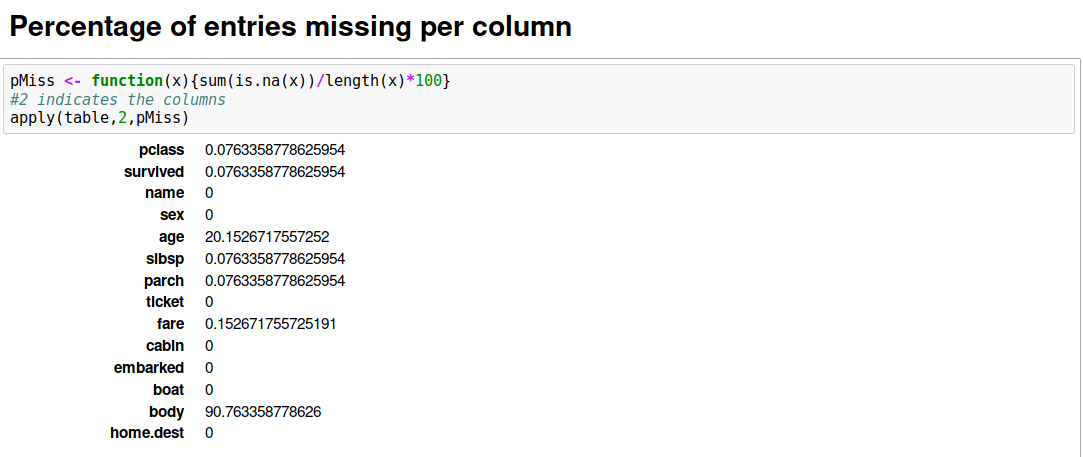
\includegraphics[width = \textwidth]{images/R2.png}
\caption{High Percentage of Missing Data}
\end{figure}
\par\noindent Then we can apply the MICE function with the right parameter in order to obtain multiple suggested values for each entry (i.e. row) where the value is missing.
\begin{figure}[htbp]
\centering
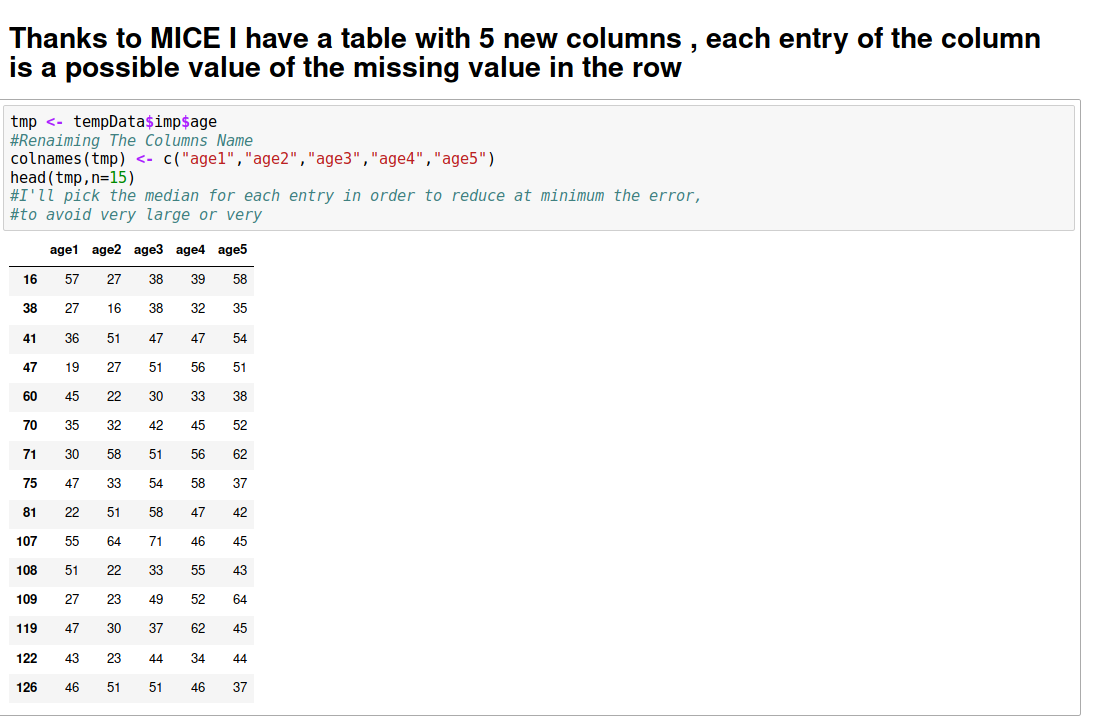
\includegraphics[width = \textwidth]{images/R3.png}
\caption{Creating Multiple Datasets}
\end{figure}
\newpage
We can easily see that we could fill the 16th entry with 5 different values. There are different techniques to choose from in order to fill the incomplete dataset, like taking into account standard error, variance, and mean of each table. We choose to fill the incomplete dataset with the median of each row, since the median is more robust than other technique against outliers.
\begin{figure}[htbp]
\centering
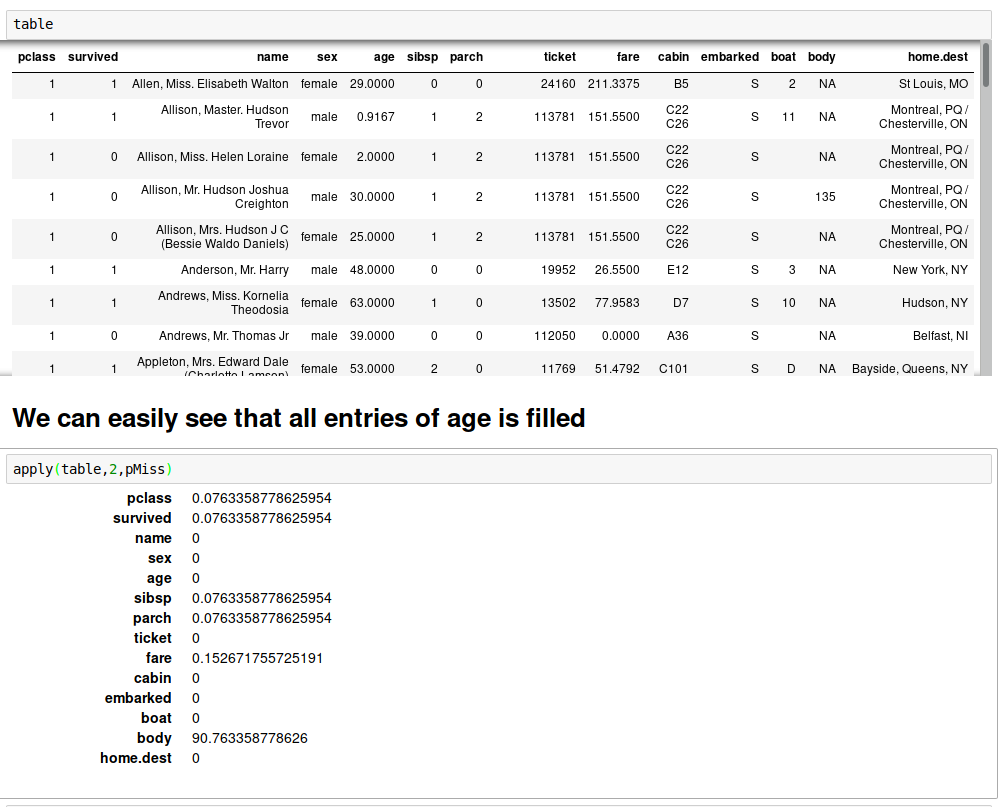
\includegraphics[width = \textwidth]{images/R4.png}
\caption{Every entry of Age now is filled-in}
\end{figure}

\par\noindent \textit{Question: } Why can Multiple Imputation be better than Single Imputation?
\par\noindent \textit{Answer: }  The problem with the Single Imputation technique is that is does not take into account randomness, it simply fills the data with already known data. For example, if in the dataset there are only "regular" values (values close to the mean), the missing data will be filled in by these "regular" value. Instead, in real cases where randomness occur, there will be some outliers that deviate a bit the variance and the standard distribution of the data. Multiple Imputation incorporates randomness, performing multiple iterations on the same entry and taking as an input a seed that helps in enhancing randomness of data.

\section{6. Conclusions}
\par\noindent We covered the theory behind missing data and some examples of how to deal with it including a Jupyter Notebook implementation available online. Discarding data (i.e. complete-case analysis) should only be used when there is very little missing data. We covered several of the single value methods including mean imputation and backward and forward filling. We reviewed the negative aspects of these methods but also when they might be used. Finally, we reviewed multiple value imputation, which takes into account the variance and uncertainty of the missing data and provided a more powerful solution worth trying.\\
\par\noindent When comparing Python and R, generally speaking, one could implement or find implementations for all methods in both languages. However, we found a more developed library for multiple value implementation in R called “MICE”. A similar library has been implemented in Python called "fancyimpute" but there is not a well-developed documentation for multiple value imputation. Therefore, this is an example for "monolingual" Python users as to what's out there. R users have a long history of well-developed tutorials and a wide-array of documentation for statistical analysis and data science.   

% citation section
\begin{thebibliography}{9}
	\bibitem{MICE}
	Azur, M. J., Stuart, E. A., Frangakis, C., \& Leaf, P. J. (2011). Multiple imputation by chained 		equations: what is it and how does it work?. International journal of methods in psychiatric research, 		20(1), 40-49. 
	
	\bibitem{Gelmann}
    Vaughn, B. K. (2008). Data analysis using regression and multilevel/hierarchical models, by Gelman, 	A., \& Hill.
	
	\bibitem{Dealingwith}
    Soley-Bori, M. (2013). Dealing with missing data: Key assumptions and methods for applied analysis. 	Boston University.
	
	\bibitem{AReviewofMethods}
	Pigott, T. D. (2001). A review of methods for missing data. Educational research and evaluation, 7(4), 		353-383.
\end{thebibliography}

\end{document}

% This is how you write code into Latex:
% \lstinputlisting[language=R,label=lst:r_code,caption=Boxplot example]{code/boxplot.R}